\documentclass[11pt]{article}

\usepackage{times}
\usepackage{alltt}
\usepackage{exam}
\usepackage{graphicx} 
\usepackage{wrapfig} 

%%%%%%%%%%%%%% 
%% Page layout
%%%%%%%%%%%%%%
\oddsidemargin 0pt
\evensidemargin 0pt
\textheight 600pt
\textwidth 469pt
\setlength{\parindent}{0em}
\setlength{\parskip}{1ex}

\begin{document}
\begin{flushright}
{\large\bf Full Name:\_\_\_\_\_\_\_\_\_\_\_\_\_\_\_\_\_\_\_\_\_\_\_\_\_\_\_\_\_\_\_\_\_\_\_\_\_\_\_\_\_ } \\[1ex]
\end{flushright}
\vspace*{0.5 in}

\setcounter{maxpage}{3}

\begin{center}
{\LARGE\bf CS 4300, Fall 2023\\ [2 ex]
Quiz 2}\\ [2 ex]
Oct 3, 2023
\end{center}

\textbf{Puzzle Scenario}

\begin{wrapfigure}{R}{0.20\textwidth}
  \vspace{-22pt}
  \begin{center}
    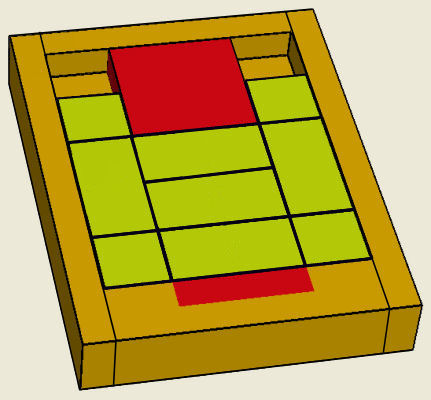
\includegraphics[width=0.20\textwidth]{jk-supercompo.jpg}
  \end{center}
  \vspace{-20pt}
  \caption{Supercompo Puzzle}
\end{wrapfigure}

The puzzle shown is a variation of slider puzzles.  Legal moves are made
by sliding a piece into an unoccupied area.  Each slide is a separate
move.  In this puzzle, the pieces have a variety of shapes.  The goal
is to move the big red piece to the bottom of the box next to the
red line on the border.  Our agent is a digital agent.  It is presented with
a digital copy of the problem in a suitable format and returns a sequence
of actions in a suitable format.

For this set of problems, consider implementing the Supercompo agent using classic search.
If you don't have sufficient information to answer any question, make your
best guess, and state why you feel it is inaccurate.

\begin{problem}{1}
  What is the maximum value of $b$, the branching factor?  Be sure to consider
  advanced states of the puzzle, not just the start state.
  \vspace*{1.5in}
\end{problem}

\begin{problem}{1}
  What is the value of $m$, the maximum tree depth?
  \vspace*{1.5in}
\end{problem}

\begin{problem}{1}
  What is the value of $d$, the depth of the shallowest goal?
  \vspace*{1.5in}
\end{problem}

\begin{problem}{1}
  Would you use tree or graph search for this problem?  Why?
  \vspace*{1.5in}
\end{problem}

\begin{problem}{1}
  Which frontier variety (e.g. DFS, DL, IDS, BFS, UC, A*, etc.) would you use?  Why?
  \vspace*{1.5in}
\end{problem}

\begin{problem}{2}
  Are your choices for the previous two questions consistent? Why or why not?
  \vspace*{1.5in}
\end{problem}


\newpage
\textbf{Micro Device Search Scenario}

A particular search problem has no heuristic available, but needs to be solved as efficiently as possible.  Analysis shows that the search tree for the problem is finite with a maximum depth of 10.  Each state has up to 3 legal actions.  The goal states are only found at the maximum depth.  Each problem instance has many goal states;  approximately 50\% of the maximum depth states are goals, spread across the maximum depth.  This search needs to take place on a micro-device, quickly finding its solutions to minimize lag times for users.  Each solution needs to be found in less than 0.5 seconds.  Because of the nature of the problem, each node takes approximately 0.001 seconds to expand.  Note: $3^{10} = 59049$.

\begin{problem}{2}

  Write the Big-O limits on the time and space complexity for BFS and DSF on this problem.  Give numbers and the formulas used to calculate them.
  
  \vspace*{2in}
  
\end{problem}

\begin{problem}{1}

  Which classic tree search strategy (not limited to BFS and DFS) would you use for this problem?
  Why?
  
  \vspace*{1in}
  
\end{problem}
\end{document}
